\documentclass{standalone}
\usepackage{tikz}
\usepackage{tkz-euclide}
\usepackage{ctex}
\setCJKmainfont{Noto Serif CJK SC}
\usepackage{mhchem,siunitx}
\usetikzlibrary{positioning}
\begin{document}
\small
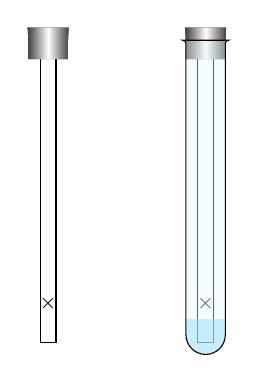
\begin{tikzpicture}[scale=1.0]
  \begin{scope}
    \draw(-0.1,-0.1)rectangle(0.1,-4);
    \fill[left color=darkgray,right color=darkgray,middle color=white](-0.26,0)--(-0.25,-0.2)--(-0.25,-0.4)--(0.25,-0.4)--(0.25,-0.2)--(0.26,0);
    \node at (0,-3.5){\scriptsize $\times$};
  \end{scope}
  \begin{scope}[xshift=2cm]
    \draw(-0.1,-0.1)rectangle(0.1,-4);
    \fill[left color=darkgray,right color=darkgray,middle color=white](-0.26,0)--(-0.25,-0.2)--(-0.25,-0.4)--(0.25,-0.4)--(0.25,-0.2)--(0.26,0);
    \node at (0,-3.5){\scriptsize $\times$};
    \fill[cyan!60!white,opacity=0.5](-0.25,-3.7)--(-0.25,-3.9)arc(180:360:0.25)--(0.25,-3.7);
    \draw[fill=cyan!10!white,fill opacity=0.4](-0.25,-0.2)--(-0.25,-3.9)arc(180:360:0.25)--(0.25,-0.2)arc(180:90:0.04)--(-0.29,-0.16)arc(90:0:0.04)--cycle;
  \end{scope}
\end{tikzpicture}
\end{document}